\documentclass{standalone}
\usepackage{tikz}
\usetikzlibrary{shapes.geometric, arrows}

\begin{document}

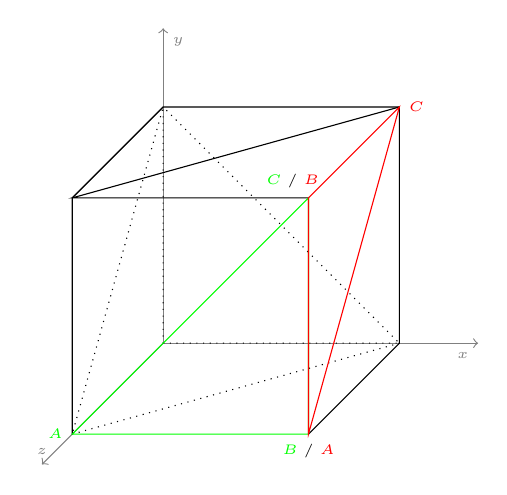
\begin{tikzpicture}

%draw the main coordinate system axes
\draw[->, gray] (0,0,0) -- (4,0,0) node[anchor=north east]{\tiny $x$};
\draw[->, gray] (0,0,0) -- (0,4,0) node[anchor=north west]{\tiny $y$};
\draw[->, gray] (0,0,0) -- (0,0,4) node[anchor=south]{\tiny $z$};




\draw[dotted] (0,0,0) -- (0,3,0) -- (0,0,3);
\draw[dotted] (3,0,0) -- (3,0,0);

\draw[green,dotted] (3,0,3) -- (3,3,3);

\draw[dotted] (0,0,0) -- (3,0,0) -- (0,3,0);
\draw (3,0,3) -- (3,0,0) -- (3,3,0) -- (0,3,0) -- (0,3,3) -- (0,0,3);
\draw  (3,3,0) -- (0,3,3) -- (3,3,3);
\draw[dotted] (0,0,3) -- (3,0,0);

\draw (0,3,3) -- (0,3,0);

\draw[green] (0,0,3) node[anchor=east] {\tiny $A$} -- (3,0,3) -- (3,3,3) -- cycle;
\draw[red] (3,0,3) node[anchor=north, green] {\tiny $B$ \color{black} / \color{red} $A$} -- (3,3,3) node[anchor=south, xshift=-0.2cm, green] {\tiny $C$ \color{black} / \color{red} $B$} -- (3,3,0) node[anchor=west] {\tiny $C$} -- cycle;

\end{tikzpicture}
\end{document}